\documentclass[lualatex]{standalone}

\usepackage{pgfplots}
\usepackage{tikz}
% \usetikzlibrary{calc,external,decorations,decorations.pathmorphing,intersections,arrows,backgrounds,positioning,arrows.meta,decorations.text,backgrounds,shapes.geometric,positioning,fit,3d,pgfplots.colormaps,intersections,tikzmark}
% \tikzset{>={Triangle[angle=35:3pt 3]}}

\usepackage{graphicx}


\begin{document}

    \begin{tikzpicture}[line width=2pt]
      \def\l{4cm}
      \node (acts) {
\includegraphics[width=3cm]{assets/logo_acts.pdf}};
      \draw[<->] (acts) --++(90:\l) node[above] {
\includegraphics[width=1.5cm]{assets/experiments/ldmx.png}};
      \draw[<->] (acts) --++(45:\l) node[above right] {
\includegraphics[width=1.5cm]{assets/experiments/alice.png}};
      \draw[<->] (acts) --++(15:\l) node[right] {
\includegraphics[width=3cm]{assets/experiments/sphenix.png}};
      \draw[<->] (acts) --++(-15:\l) node[right] {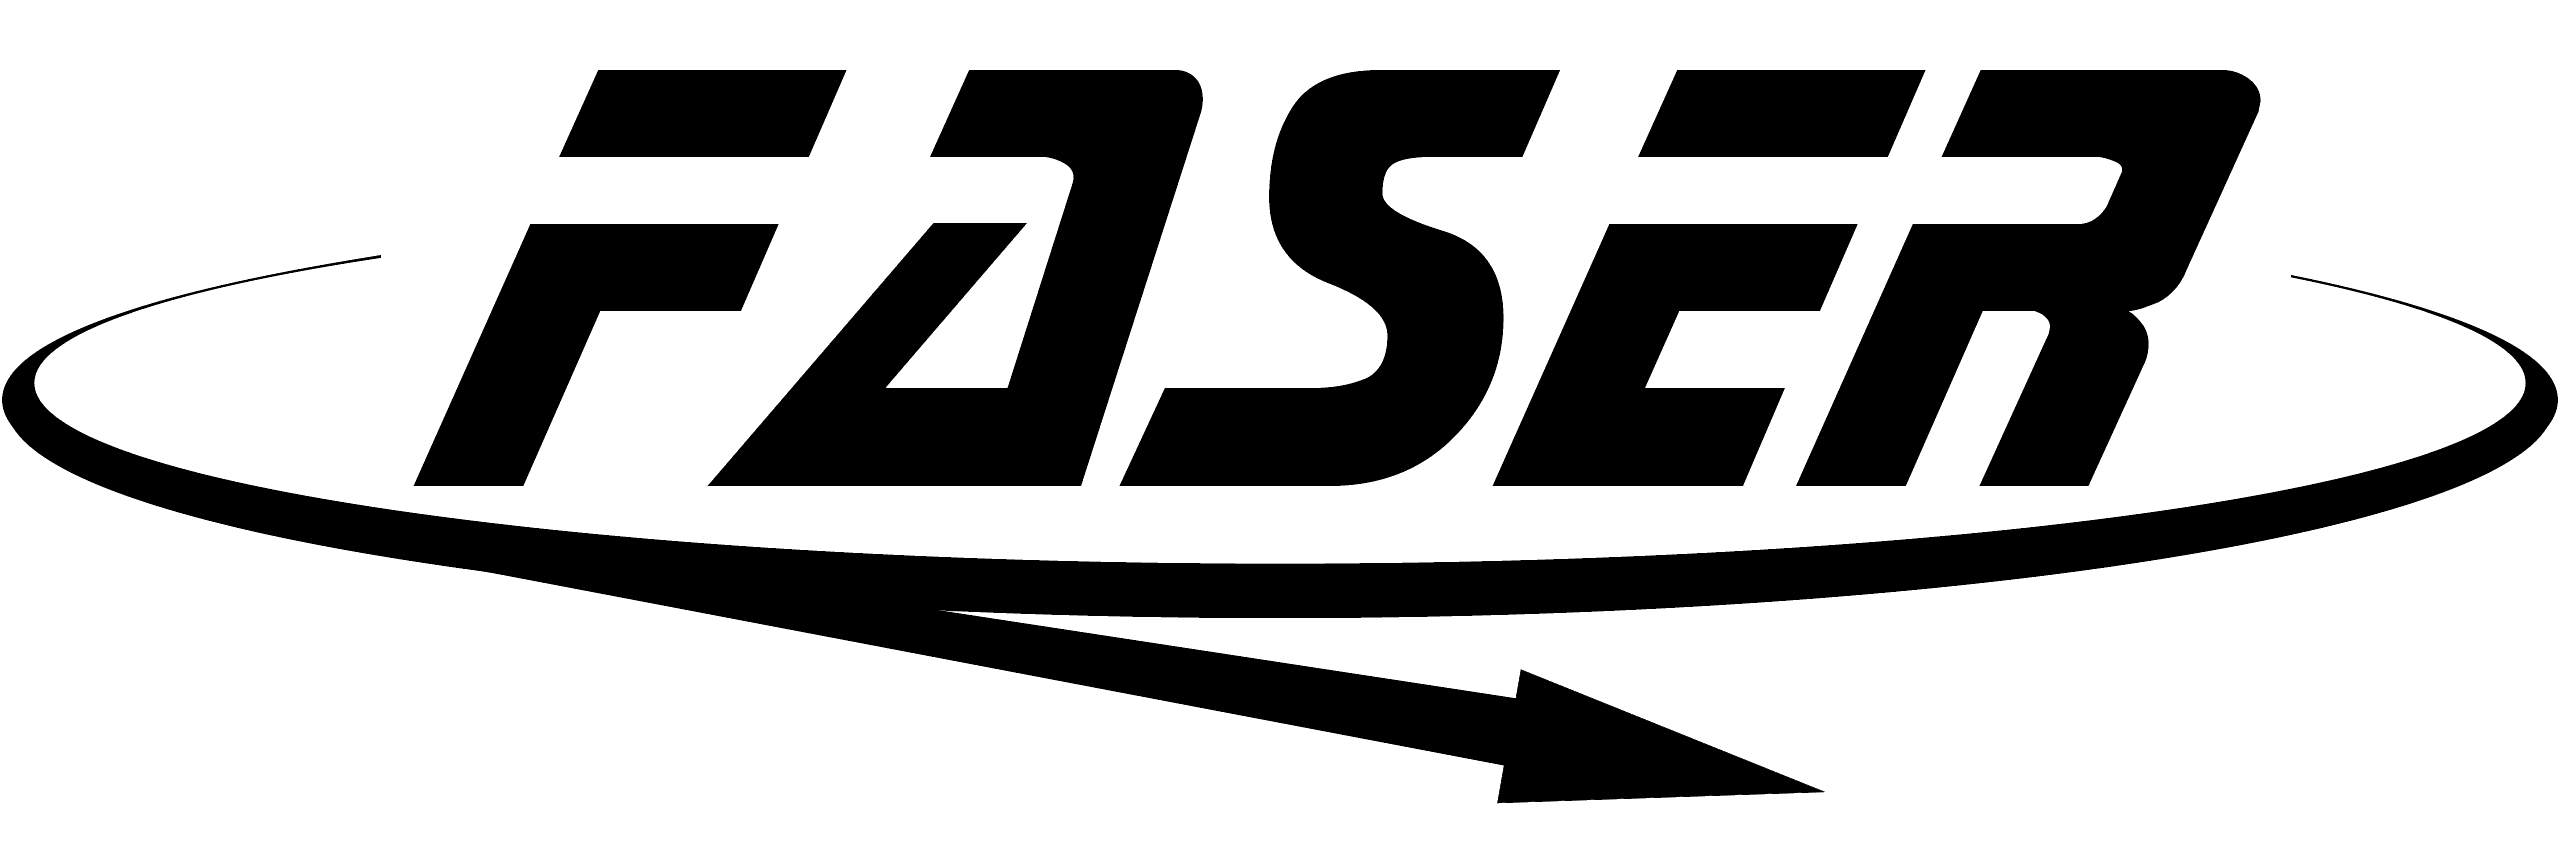
\includegraphics[width=3cm]{assets/experiments/faser.png}};

      \draw[<->] (acts) --++(-135:\l) node[below left] {
\includegraphics[width=2cm]{assets/experiments/stcf.png}};
      \draw[<->] (acts) --++(-105:\l) node[below] {\LARGE Lohengrin};
      \draw[<->] (acts) --++(-40:\l) node[below right] {
\includegraphics[width=3cm]{assets/experiments/luxe.jpg}};
      \draw[<->] (acts) --++(-66:\l) node[below] {\LARGE NA60+};

      \draw[<->] (acts) --++(-165:\l) node[below left] {
\includegraphics[width=2.5cm]{assets/experiments/cepc.png}};
      \draw[<->] (acts) --++(165:\l) node[left] {
\includegraphics[width=3cm]{assets/experiments/epic.png}};
      \draw[<->] (acts) --++(135:\l) node[above left] {
\includegraphics[width=2cm]{assets/experiments/atlas.png}};
    \end{tikzpicture}

\end{document}
